\documentclass[12pt,a4paper,twoside]{article}
%\documentclass[12pt,a4paper,twocolumn,twoside]{article}
\usepackage[utf8]{inputenc}
\usepackage[english]{babel}
\usepackage{amsmath}
\usepackage{amsfonts}
\usepackage{amssymb}
\usepackage{graphicx}
\usepackage{parcolumns}
\usepackage[left=2.cm,right=2.cm,top=2.cm,bottom=2.cm]{geometry}
\usepackage[final]{pdfpages} %serve per aggiungere altre pagine pdf al file
\usepackage{siunitx}

\author{Davide Bazzanella}
\title{Improving phase-matching of FWM with temperature}

\pagenumbering{roman}	% numeration in roman numbers
\begin{document}

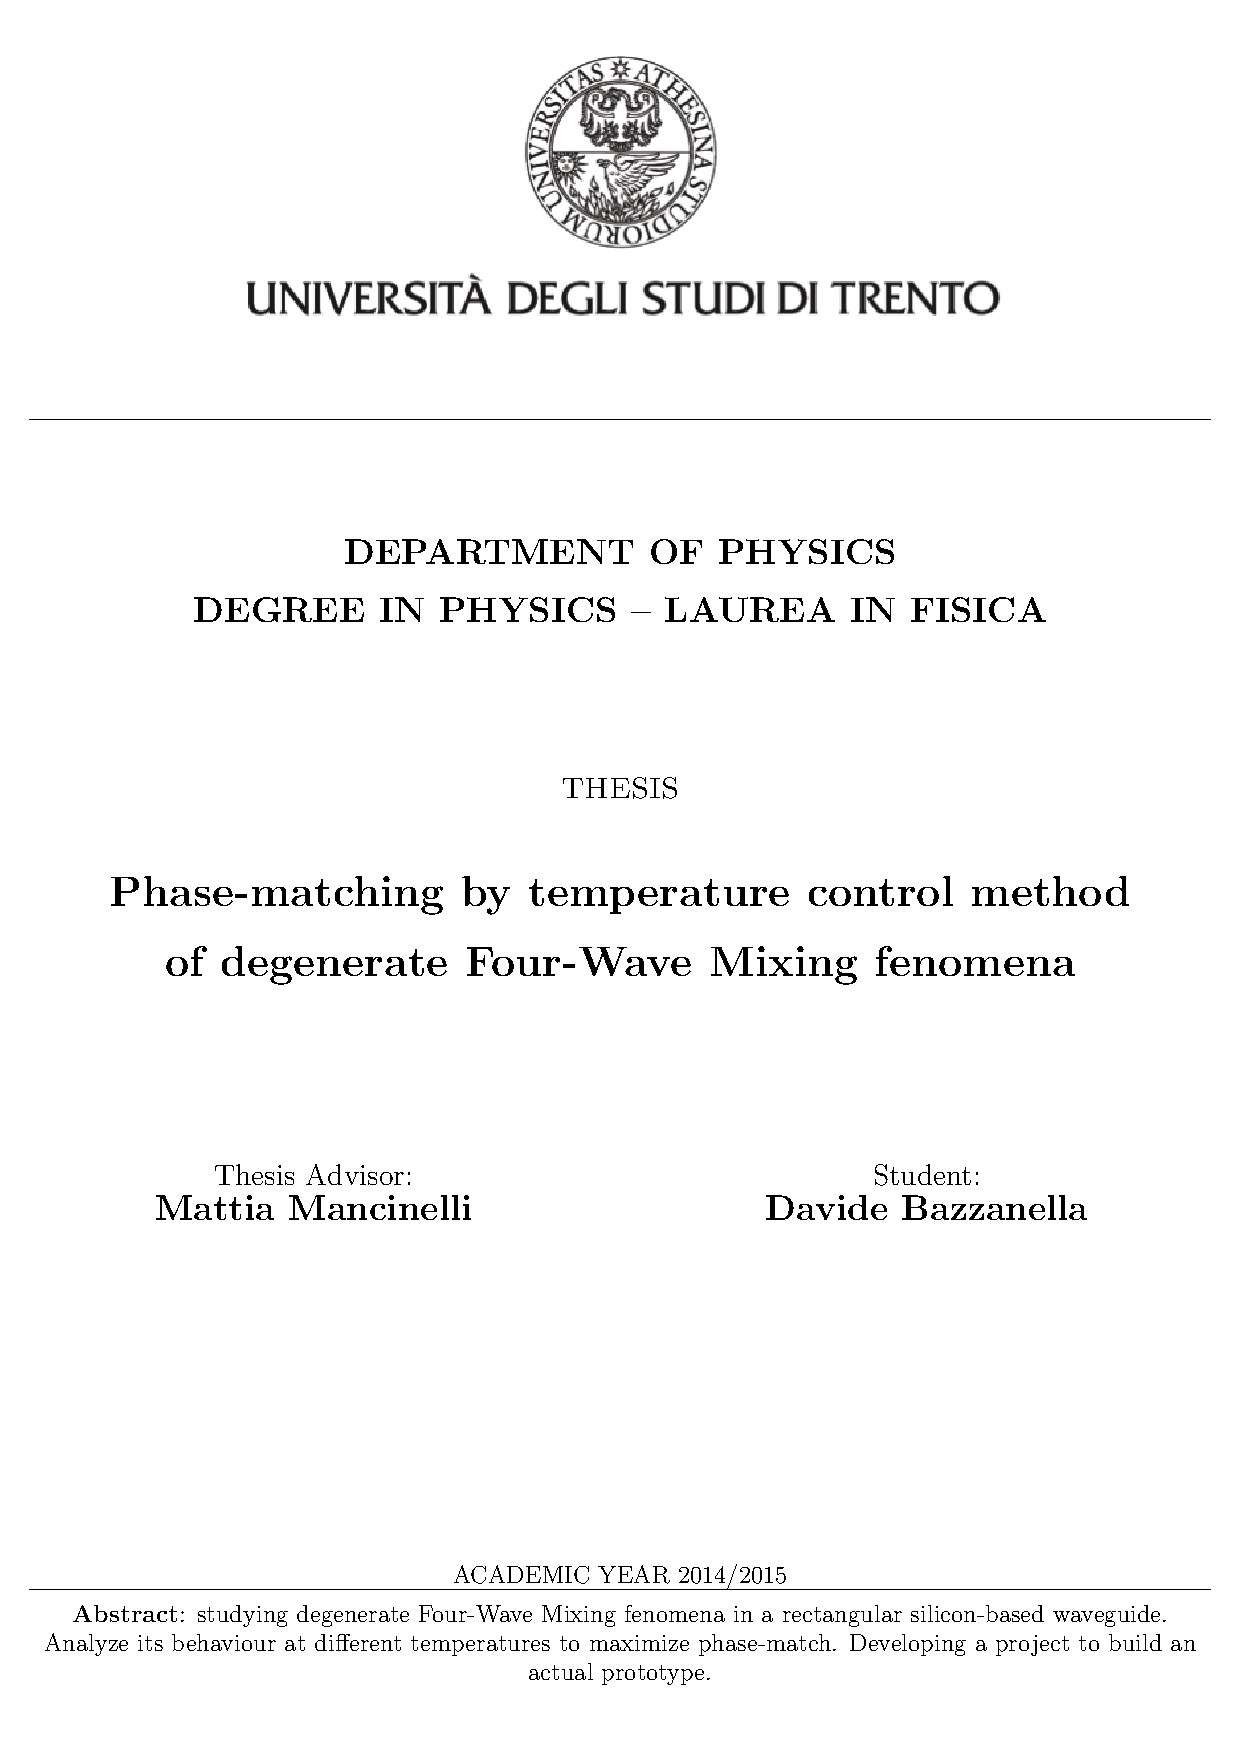
\includepdf[pages={1}]{intestazione.pdf} % \documentclass[11pt,a4paper]{article}
\usepackage[utf8]{inputenc}
\usepackage[english]{babel}
\usepackage{amsmath}
\usepackage{amsfonts}
\usepackage{amssymb}
\usepackage{graphicx}
\usepackage{parcolumns}
\usepackage[left=0.5cm,right=.5cm,top=.5cm,bottom=.5cm]{geometry}

\begin{document}

\begin{titlepage}
\begin{center}

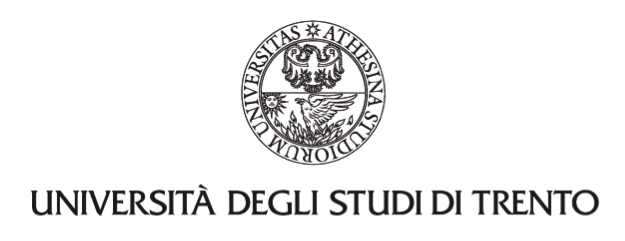
\includegraphics[width=0.7\textwidth]{unitn_logo.png}~\\[1.2cm]

\hrule
$$$$
$$$$

\textsc{\LARGE \textbf{DEPARTMENT OF PHYSICS}}\\[0.5cm]
\textsc{\LARGE \textbf{DEGREE IN PHYSICS – LAUREA IN FISICA}}\\[2.5cm]
\textsc{\Large THESIS}\\[1.3cm]

{ \huge \bfseries Phase-matching by temperature control method}\\
[0.5cm]
{ \huge \bfseries of degenerate Four-Wave Mixing fenomena}\\
[3.0cm]

% ATTENZIONE! Ha bisogno del pacchetto parcolumns per funzionare
\begin{parcolumns}{2}
   \colchunk{\Large Thesis Advisor:\\ \LARGE \textbf{Mattia Mancinelli}}
   \colchunk[2]{\Large Student:\\ \LARGE \textbf{Davide Bazzanella}}
\end{parcolumns}
$$$$
$$$$
$$$$
$$$$
$$$$
$$$$
$$$$
$$$$

\large ACADEMIC YEAR 2014/2015
\hrule
\vfill
\textbf{Abstract}: studying degenerate Four-Wave Mixing fenomena in a rectangular silicon-based waveguide. Analyze its behaviour at different temperatures to maximize phase-match. Developing a project to build an actual prototype.

\vfill

{\large}

\end{center}
\end{titlepage}

\end{document}

\cleardoublepage 
\setcounter{page}{3}
\tableofcontents

\cleardoublepage
\pagenumbering{arabic}

\section{Introduction}
\subsection{Motivation}
In my scholastic career I approached the study of optics in an elective course of my third year of undergraduate academic degree.
I became very interested in the subject, in particular because of the potential developement of photonics for communication and computing.
I discussed different topics with the professors and some researchers.
One of the researcher, who would later become my advisor, suggested me a few interesting topics in guided-wave optics which could be studied as a undergraduate thesis.

I chose to study the temperature behaviour of silicon waveguides.
The reason of the choice is that there are always discrepancies between the design of silicon objects and their actual production by the factory.
The aim of the study is to exploit behaviour of silicon to correct these possible production defects of the materials.

The study is focused on a silicon-based waveguide with a silicon ($\mathrm{Si}$) core of rectangular section and a silica ($\mathrm{Si0}_2$) cladding.
The purpose of the waveguide is to generate light through a partial degenerate Four-Wave Mixing phenomenon.

\subsection{Partially degenerate Four-Wave Mixing}
Four-Wave Mixing (FWM) is a nonlinear optical effect due to the susceptibility of silicon.
Silicon is an isotropic material and therefore second order susceptibility $\chi^{(2)}$ (almost) vanishes.
Third order susceptibility $\chi^{(3)}$, on the other hand, is non-zero and is responsible among the other effects for FWM, which is indeed a third order phenomenon.

In general FWM implies the mix of four waves of different frequency.
Partial degenerate FWM, instead, is a specific case in which two waves have the same frequency and are considered as one (pump).
Therefore it is about the pump wave and a second weaker one (signal) which generate a third wave (idler) of frequency different from that of the former two.

\section{Electromagnetic waves in dielectric media}

**** 	pg 156 saleh or chp 2 agrawal
\vspace{12pt}

To understand electromagnetic phenomena the starting point is the well known Maxwell's equations:
\begin{subequations}
\begin{align}
	\nabla \times \textbf{E} &= -\frac{\partial \textbf{B}}{\partial t} \\
	\nabla \times \textbf{H} &= \textbf{J} + \frac{\partial \textbf{D}}{\partial t} \\
	\nabla \cdot \textbf{D} &= \rho_{\mathrm{f}} \\
	\nabla \cdot \textbf{B} &= 0
\end{align}
\label{eq_maxwell}
\end{subequations}
where \textbf{E} and \textbf{H} are electri and magnetic field vectors and \textbf{D} and \textbf{B} are corresponding electric and magnetic flux densities. \textbf{J} is the current density vector and $\rho_{\mathrm{f}}$ is the free charge density.
In dielectric media, such as silicon, we can also consider $\textbf{J} = 0$ and $\rho_\mathrm{f} = 0$.

\textbf{D} and \textbf{B} are related to the electromagnetic fields through the relations:
\begin{subequations}
\begin{align}
	\textbf{D} &= \varepsilon_0 \textbf{E} + \textbf{P} \\
	\textbf{H} &= \mu_0 \textbf{H} + \textbf{M}	
\end{align}
\end{subequations}
where $\varepsilon_0$ is the vacuum permittivity, $\mu_0$ is the vacuum permeability, and \textbf{P} and \textbf{M} are the induced electric and magnetic polarizations repectively.
For a nonmagnetic medium, as in our case, $\textbf{M} = 0$.

A linear dielectric medium is characterized by a linear relation between the polarization density and the electric field:
\begin{equation}
\textbf{P} = \varepsilon_0 \chi \textbf{E}
\end{equation}
where $\chi$ is the susceptibility of the medium and $\varepsilon_r \equiv 1+\chi$ is the relative dielectric constant.

Taking the curl of eq (\ref{eq_maxwell}a) and substituting in it eq (\ref{eq_maxwell}c) it leads to the Helmholtz equation:
\begin{equation}
\nabla^2 \textbf{E} - \frac{1}{c^2}\frac{\partial^2 \textbf{E}}{\partial t^2} = \mu_0\frac{\partial^2 \textbf{P}}{\partial t^2}
\label{eq_helm_P}
\end{equation}
where $c = 1/\sqrt{\mu_0 \varepsilon_0}$ is the speed of light in vacuum.

Defining the refractive index $n \equiv \sqrt{\varepsilon_r}$ of the material the previous equation (\ref{eq_helm_P})
\begin{equation}
\nabla^2 \textbf{E} - \frac{n^2}{c^2}\frac{\partial^2 \textbf{E}}{\partial t^2} = 0
\end{equation}
Moreover, $n$ represent the ratio between the speed of light in vacuum and in the material $n = c/v$.

In linear optics the technology for trasmitting a light wave by confining it in a finite space is the guided-wave optics.
The instruments employed for achieving such purpose are called waveguides.

\subsection{Silicon waveguides}
In a ray-optics picture, silicon waveguides are dielectric waveguides and make use of the interface between two media with different refractive index.
Precisely they exploit the phenomenon of total internal reflection: if a propagating wave reaches a boundary between two mediums, one with higher refractive index ($n_H$) and another with lower refractive index ($n_L$), with an angle of incidence greater than the \textit{critical angle}, then the wave is completely reflected in the first medium.
%accorciare la precedente frase%
Angles are defined relative to the normal vector of the interface and the critical angle can be obtained by the Snell law:

$$	\theta_C = \arcsin \left( \frac{n_L}{n_H} \right)$$

Silicon waveguides are composed by core and cladding \textbf{(?)}. %is called cladding only for fiber or also for slab/strip wg?
The former is the higher refractive index medium in which the wave is confined, the latter is the lower refractive index medium which surrounds the core, thus creating the interface. Theoretically the cladding could also be vacuum.

\vspace{18pt}
**** ripresa delle eq di maxwell?
\vspace{12pt}

Considering an ideal dielectric waveguide (no absorption) and the total field distribution as sum of transverse electromagnetic (TEM) plane waves is possible to study the propagation of the wave along the waveguide with an electromagnetic analysis.
Furthermore it can be shown that not all field distribution are transmitted through the waveguide without energy loss \textbf{(?)}.

% Modes are fields that maintain the same transverse distribution and polarization at all locations along the waveguide axis.
Those field distributions which maintain the same transverse distribution and polarization at all locations along the waveguide axis are called modes.
These modes can be categorized in two main groups, depending on the polarization of the wave: transverse electric (TE) modes and transverse magnetic (TM) modes, which have respectively the electric and magnetic field transverse to the waveguide axis.

Both TE and TM modes can be again classified by their order, that is proportional to the number of maxima of the modulus of the electric and magnetic fields in the core section.
The first order has only one maximum at the center of the core, the second order has two maxima placed simmetrically from the center and so on.

Moreover it is noteworthy that the field distributions of odd orders are even functions and those of even order are odd functions.

\begin{figure}[ht]
	\centering
	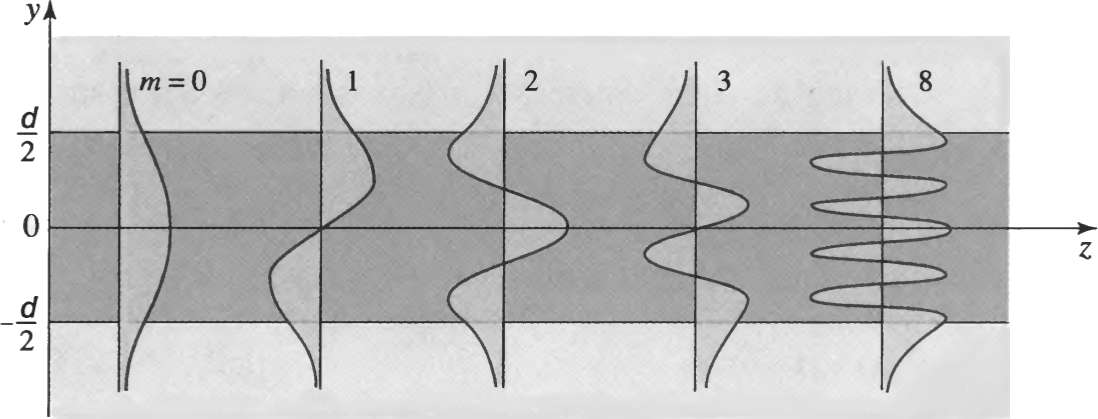
\includegraphics[width=.75\textwidth]{1D_fields.png}
	\label{fig_1dmodes}
	\caption{graphical rapresentation of field distribution of 1D modes}
\end{figure}

\vspace{18pt}
****		\textit{effective index}
\vspace{12pt}

A very important parameter of each mode is its \textit{propagation constant} $\beta$, defined as the component of the wavevector $k$ in the waveguide axis:
\begin{equation}
\beta \equiv k_z
\end{equation}

Higher-order modes travel with smaller propagation constants.
For a 1D slab waveguide $\beta$ has a simple relation with the bounce angles $\theta_m$, which are quantized between $0$ and $\bar{\theta}_C = \pi - \theta_C$:
$$\beta_m = n_H k_0 \cos \theta_m$$

From the propagation constant, we can also define the refractive index relative to the propagation mode, called \textit{effective index}:
\begin{equation}
\beta = k_0 n_{eff} \quad \Rightarrow \quad n_{eff} \equiv \frac{\beta}{k_0}
\end{equation}

Its value is between the higher index of the core and lower one of the cladding.
Again, for the 1D slab waveguide case, the effective index can be rewritten as in the following formula:
$$ n_{eff} \equiv n_H \cos \theta_m$$

\subsection{Rectangular dielectric waveguides}
In general, in a rectangular dielectric waveguide the classification of modes need two indexes because we have two degrees of freedom.
For our purpose, due to the thin geometry of the core, modes with the higher effective index are fundamental modes in the height axis.
Only one significant index is then left to describe the order of modes.

\begin{figure}[ht]
	\centering
	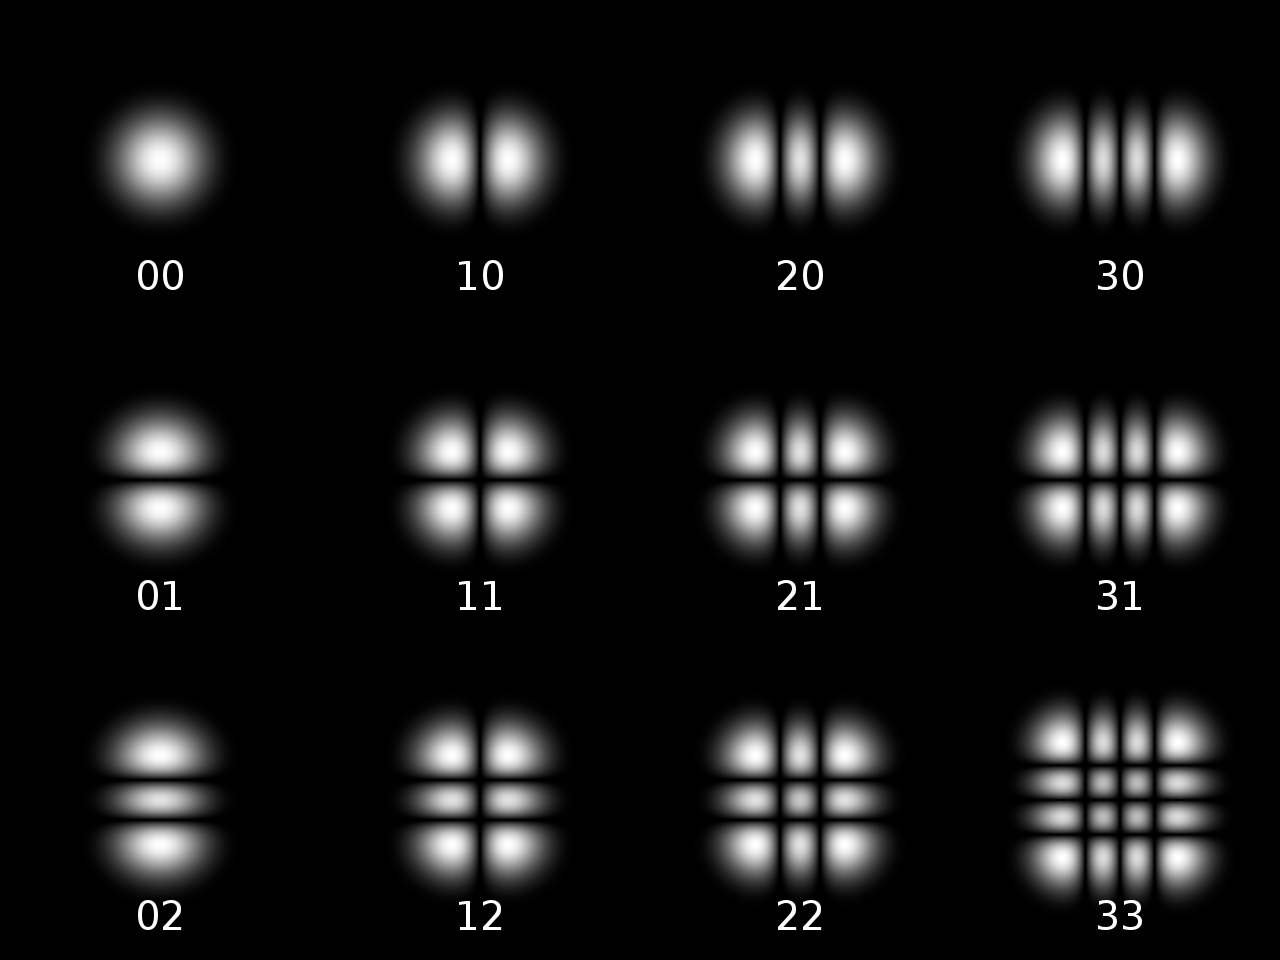
\includegraphics[width=.5\textwidth]{2Dmodes.png}
	\label{fig_2dmodes}
	\caption{graphical rapresentation of field distribution of 2D modes}
\end{figure}

\section{Non-linear optics}
A nonlinear dielectric medium is characterized by a nonlinear relation between P and E, such as
\begin{equation}
\textbf{P} = \varepsilon_0 \left( \chi^{(1)} \cdot \textbf{E} + \chi^{(2)} : \textbf{E}^2 + \chi^{(3)} \vdots \textbf{E}^3 + \cdots \right)
\end{equation}
which originates from the behaviour of bound electrons.

In everyday condition linear effects are much larger than nonlinear ones.
The relation between $\mathrm{P}$ and $\mathrm{E}$ becomes nonlinear when $\mathrm{E}$ has a value comparable to interatomic electric fields, which are typically $\sim 10^5-10^8$ \si{\V\per\m}.

For an isotropic medium the second order term is zero (in the dipole approximation) and this is our scenario.
Thus the dominant nonlinearity is the third order and the material is called a Kerr medium.

\subsection{Third order effect: Four-Wave Mixing}
Many processes are result of third order nonlinearities: Third-Harmonic Generation (THG), Kerr Effect, Cross-phase modulation (XPM), Self-phase modulation (SPM) and Four-Wave Mixing (FWM).

The parametric process of Four-Wave Mixing originates from the third order nonlinear response of a material to an electromagnetic field and involves interaction among four optical waves.

\vspace{18pt}
****		è necessario verificare conservazione di energia e momento
\vspace{12pt}

In order to be efficient, the parametric process needs to verify both the conservation of energy and momentum.
\begin{equation}
\omega_1 + \omega_2 = \omega_3 + \omega_4
\end{equation}
\begin{equation}
\beta_1 + \beta_2 = \beta_3 + \beta_4
\end{equation}
%\Delta k = \beta_3 + \beta_4 - \beta_1 - \beta_2

\section{Simulating and coding}

To understand the behaviour of the waveguide, it is necessary to first know how waves of different frequency are transmitted through the waveguide.
We chose to simulate the modes with temperature and frequency as a parameters.

Our aim was to develop a model to work with an infrared laser pump with $\lambda_{p} = \SI{1.55}{\um}$.
We narrowed our simulations to a frequency gap centered in $\omega_p = 2\pi \nu_p = 2\pi c / \lambda_{p}$.
The gap chosen was precisely $[\SI{1.45}{\um} ,\, \SI{1.65}{\um}]$ or the equivalent $[\SI{182}{\THz} ,\, \SI{207}{\THz}]$.

The reason for this choice is that silicon is transparent at these wavelenght and also for the availability of laser that emit at the specific wavelenght.

\vspace{18pt}
****
\vspace{12pt}

Our data output was therefore the field distribution and effective index for a number of modes for each parametric configuration.

The next step was to classify these data depending on the order and type (TE or TM) of the modes.
We achieved this by analyzing the maxima of the field distributions.
We obtained then a well organized data matrix filled with the value of effective index for each combination of parameters.

\subsection{Data processing}
Starting from raw data consisting of the effective index for each parametric configuration, we fitted them with a polinomial function of frequency $\omega = 2\pi \nu$ and temperature $T$, obtaining:
$$n_{eff} = f_{mt,\,mo} \left( \omega, T \right)$$
where $mt$ and $mo$ means respectively \textit{mode type} (TE or TM) and \textit{mode order} (1, 2, 3, ...)

\vspace{18pt}
************************************

\subsubsection*{Order combination}

Due to the intrinsic symmetry of the problem (and thus of the integrals) not all combinations of orders can produce FWM.
Only those in which the sum of the orders is an even number are interesting.
To narrow the possible sets, we chose to permit only full TE or full TM  combinations.

We eventually obtained a list of combinations, for each of which we verified the conservation of energy and momentum.


$$\omega_1 = \omega_2 = \omega_P$$
$$\omega_I = 2\omega_P - \omega_S$$
$$\Omega_S = \omega_1 + \omega_3 = \omega_4 - \omega_1$$
where we assume $\omega_3 < \omega_4$.
$$\Omega_S = |\omega_P - \omega_I| = |\omega_S - \omega_P|$$

$$\Delta k = \beta_3 + \beta_4 - 2\beta_1$$

$$L_{coh} = \frac{2\pi}{|\Delta k|}$$



\section{Prototyping}

\subsection{Heater configurations}
In order to achieve a greater effect from the different temperature, we tried to move the heater from over the center of the core to the side.
This operation was intended to increase the difference of behaviour between low and high orders.
\subsection{Different geometries}

\section{Conclusion}

\cleardoublepage
\begin{thebibliography}{9}
\bibitem{agrawal} G. Agrawal. Nonlinear Fiber Optics, 5th edition. 2013
\bibitem{saleh} B. E. A. Saleh, M. C. Teich. Fundamentals of photonics, 2nd edition. 2007
\end{thebibliography}
\end{document}
% Ref. \cite{agrawal}